
\textbf{Pour cette première partie, aucune justification n'est demandée et une seule réponse est possible par question. Pour chaque question, reportez son numéro sur votre copie et indiquez votre réponse.}

\subsubsection*{Question 1}
Donner un ordre de grandeur de $101 \times 99$ :

\textbf{a.} 100\hfill \textbf{b.} 1\,000\hfill \textbf{c.} 10\,000\hfill \textbf{d.} 100\,000

\subsubsection*{Question 2}
Un prix augmente de 20\% puis diminue de 20\%. Après ces deux évolutions, on peut affirmer que :

\textbf{a.} Le prix est égal à sa valeur de départ. \\
\textbf{b.} Le prix est strictement supérieur à sa valeur de départ. \\
\textbf{c.} Le prix est strictement inférieur à sa valeur de départ. \\
\textbf{d.} On ne peut pas savoir : cela dépend de la valeur de départ.

\subsubsection*{Question 3}
Par combien faut-il multiplier une quantité positive pour que celle-ci diminue de 2,3\% ?

\textbf{a.} 1,23\hfill \textbf{b.} 0,977\hfill \textbf{c.} 0,77\hfill \textbf{d.} 1,023

\subsubsection*{Question 4}
Dans un lycée, 50 élèves étudient le Grec, ce qui représente 4\% du nombre d'élèves inscrits dans ce lycée. \\
Le nombre d'élèves inscrits dans ce lycée est égal à :

\textbf{a.} 2\hfill \textbf{b.} 200\hfill \textbf{c.} 125\hfill \textbf{d.} 1\,250

\subsubsection*{Question 5}
Le volume d'un glacier diminue de 3\% chaque année. \\
Si $V(n)$ désigne le volume du glacier pour l'année $n$ on a :

\textbf{a.} $V(n + 1) = V(n) - 0,03$\hfill \textbf{b.} $V(n + 1) = 0,03 \times V(n)$

\textbf{c.} $V(n + 1) = 0,97 \times V(n)$\hfill \textbf{d.} $V(n + 1) = V(n) - 0,97$

\bigskip

\begin{minipage}[t]{0.6\textwidth}
\subsubsection*{Question 6}
Dans un repère du plan on a représenté une droite. \\
Le coefficient directeur de cette droite est égal à :

\textbf{a.} $-3$\hfill \textbf{b.} $-1$\hfill \textbf{c.} $2$\hfill \textbf{d.} $3$
\end{minipage}
\hfill
\begin{minipage}[t]{0.35\textwidth}
\vspace{0pt}
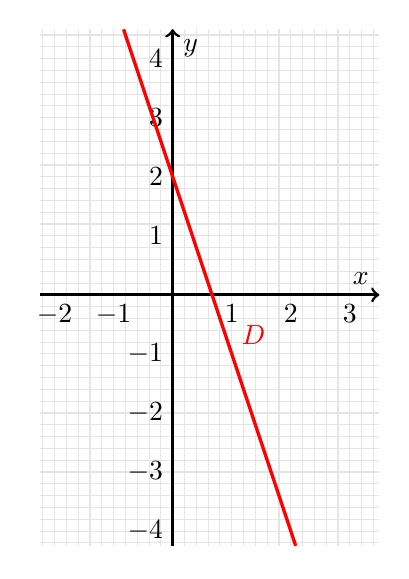
\begin{tikzpicture}[scale=0.75]
\def\xmin{-2.25}
\def\xmax{3.5}
\def\ymin{-4.25}
\def\ymax{4.5}
\pgfmathsetmacro\xymin{(\ymin - 2) / -3}
\pgfmathsetmacro\xymax{(\ymax - 2) / -3}
\draw[gray] (\xmin,\ymin) grid (\xmax,\ymax);
\foreach \x in {-2.2,-2.0,...,\xmax} {
    \draw[gray!20] (\x,\ymin) -- (\x,\ymax);
}
\foreach \y in {-4.2,-4.0,...,\ymax} {
    \draw[gray!20] (\xmin,\y) -- (\xmax,\y);
}
\draw[->, line width=1pt] (\xmin,0) -- (\xmax,0) node[above left] {$x$};
\draw[->, line width=1pt] (0,\ymin) -- (0,\ymax) node[below right] {$y$};
\foreach \x in {-2,-1} {
    \node[below] at (\x,0) {$\x$};
}
\foreach \x in {1,...,3} {
    \node[below] at (\x,0) {$\x$};
}
\foreach \y in {-4,-3,-2,-1} {
    \node[left] at (0,\y) {$\y$};
}
\foreach \y in {1,...,4} {
    \node[left] at (0,\y) {$\y$};
}
\draw[red, very thick] plot[domain=\xymin:\xymax, samples=100] (\x, {-3*\x + 2});
\node[above right, text=red] at (1, -1) {$D$};
\end{tikzpicture}
\end{minipage}

\subsubsection*{Question 7}
Dix stylos coûtent en tout 13 euros. \\
Le prix de trois stylos est égal à :

\textbf{a.} 3,60 euros\hfill \textbf{b.} 6,90 euros\hfill \textbf{c.} 3,90 euros\hfill \textbf{d.} 6,50 euros

\subsubsection*{Question 8}
Une athlète parcourt 1 km en 5 minutes. Quelle est sa vitesse moyenne ?

\textbf{a.} 8 km/h\hfill \textbf{b.} 10 km/h\hfill \textbf{c.} 12 km/h\hfill \textbf{d.} 14 km/h

\subsubsection*{Question 9}
Sur 60 personnes présentes à une exposition, on distingue trois groupes :
\begin{itemize}[label=\textbullet]
\item groupe A : 30 personnes
\item groupe B : 12 personnes
\item groupe C : les autres.
\end{itemize}
Quelle représentation décrit la situation ?

\textbf{a.}

\begin{tikzpicture}[scale=0.75]
    \fill[blue!20] (0,0) -- (210:1.5cm) arc (210:330:1.5cm) -- cycle;
    \fill[black] (0,0) -- (330:1.5cm) arc (330:450:1.5cm) -- cycle;
    \fill[gray] (0,0) -- (90:1.5cm) arc (90:210:1.5cm) -- cycle;
    \draw[white, line width=0.75mm] (0,0) -- (90:1.5cm);
    \draw[white, line width=0.75mm] (0,0) -- (210:1.5cm);
    \draw[white, line width=0.75mm] (0,0) -- (330:1.5cm);
\end{tikzpicture}
\hfill
\textbf{b.}

\begin{tikzpicture}[scale=0.75]
    \fill[blue!20] (0,0) -- (198:1.5cm) arc (198:270:1.5cm) -- cycle;
    \fill[black] (0,0) -- (270:1.5cm) arc (270:450:1.5cm) -- cycle;
    \fill[gray] (0,0) -- (90:1.5cm) arc (90:198:1.5cm) -- cycle;
    \draw[white, line width=0.75mm] (0,0) -- (90:1.5cm);
    \draw[white, line width=0.75mm] (0,0) -- (198:1.5cm);
    \draw[white, line width=0.75mm] (0,0) -- (270:1.5cm);
\end{tikzpicture}
\hfill
\textbf{c.}

\begin{tikzpicture}[scale=0.75]
    \fill[blue!20] (0,0) -- (300:1.5cm) arc (300:342:1.5cm) -- cycle;
    \fill[black] (0,0) -- (342:1.5cm) arc (342:450:1.5cm) -- cycle;
    \fill[gray] (0,0) -- (90:1.5cm) arc (90:300:1.5cm) -- cycle;
    \draw[white, line width=0.75mm] (0,0) -- (90:1.5cm);
    \draw[white, line width=0.75mm] (0,0) -- (300:1.5cm);
    \draw[white, line width=0.75mm] (0,0) -- (342:1.5cm);
\end{tikzpicture}
\hfill
\textbf{d.}

\begin{tikzpicture}[scale=0.75]
    \fill[blue!20] (0,0) -- (180:1.5cm) arc (180:270:1.5cm) -- cycle;
    \fill[black] (0,0) -- (270:1.5cm) arc (270:450:1.5cm) -- cycle;
    \fill[gray] (0,0) -- (90:1.5cm) arc (90:180:1.5cm) -- cycle;
    \draw[white, line width=0.75mm] (0,0) -- (90:1.5cm);
    \draw[white, line width=0.75mm] (0,0) -- (180:1.5cm);
    \draw[white, line width=0.75mm] (0,0) -- (270:1.5cm);
\end{tikzpicture}

\subsubsection*{Question 10}
On considère les deux séries ci-dessous.

Série A : 9 ; 10 ; 10 ; 11 \hfill Série B : 7 ; 10 ; 10 ; 13

Une seule des quatre propositions suivantes est vraie.

\textbf{a.} La moyenne de la série A est strictement supérieure à la moyenne de la série B. \\
\textbf{b.} La moyenne de la série B est strictement supérieure à la moyenne de la série A. \\
\textbf{c.} L'écart-type de la série A est strictement supérieur à l'écart-type de la série B. \\
\textbf{d.} L'écart-type de la série B est strictement supérieur à l'écart-type de la série A.

\subsubsection*{Question 11}
Le volume $V$ d'un cylindre de hauteur $h$ et de rayon $r$ est égal à

\[V = \pi r^2 h.\]

On cherche à isoler $h$. On a :

\textbf{a.} $h = \sqrt{\dfrac{V}{\pi r^2}}$\hfill \textbf{b.} $h = \dfrac{\pi r^2}{V}$\hfill \textbf{c.} $h = \dfrac{V}{\pi r^2}$\hfill \textbf{d.} $h = \dfrac{r^2}{\pi V}$

\bigskip

\begin{minipage}[t]{0.5\textwidth}
\subsubsection*{Question 12}
Soit $f$ une fonction définie sur l'intervalle $[-4~;~4]$ dont la représentation graphique est donnée ci-contre. \\
L'ensemble $S$ des solutions de l'équation $\mbox{f(x) = 0}$ est :

\textbf{a.} $S = \{0\}$\hfill \textbf{b.} $S = [-3~;~2]$\hfill

\textbf{c.} $S = \{-3~;~-1~;~1~;~2\}$\hfill \textbf{d.} $S = \{1,5\}$
\end{minipage}
\hfill
\begin{minipage}[t]{0.45\textwidth}
\vspace{0pt}
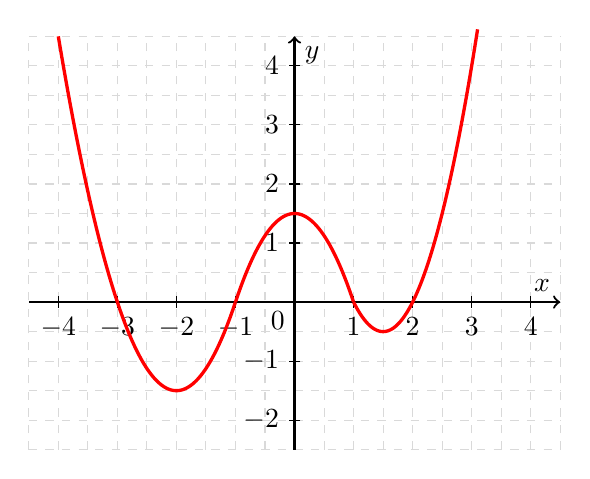
\begin{tikzpicture}[scale=0.75]
\draw[gray!30, dashed] (-4.5,-2.5) grid[step=0.5] (4.5,4.5);
\draw[->, thick] (-4.5,0) -- (4.5,0) node[above left] {$x$};
\draw[->, thick] (0,-2.5) -- (0,4.5) node[below right] {$y$};
\foreach \x in {-4,-3,..., -1,1,2,...,4} \draw (\x,0.1) -- (\x,-0.1) node[below] {$\x$};
\foreach \y in {-2,-1,1,2,...,4} \draw (0.1,\y) -- (-0.1,\y) node[left] {$\y$};
\node[below left] at (0,0) {0};
\draw[red, very thick, smooth, samples=100, domain=-4:-1] plot(\x, {1.5*(\x)^2 + 6*(\x) + 4.5});
\draw[red, very thick, smooth, samples=100, domain=-1:1] plot(\x, {-1.5*(\x)^2 + 1.5});
\draw[red, very thick, smooth, samples=100, domain=1:3.1] plot(\x, {2*(\x)^2 - 6*(\x) + 4});
\end{tikzpicture}
\end{minipage}




\begin{center}
\textbf{\large DEUXIÈME PARTIE (14 pts)}
\end{center}

